\everymath{\displaystyle}
\documentclass{beamer}
% \documentclass[handout]{beamer}

%\usepackage[pdftex]{color,graphicx}
\usepackage{amsmath,amssymb,amsfonts}

\mode<presentation>
{
  % \usetheme{Darmstadt}
  % \usetheme[hideothersubsections]{Hannover}
  % \usetheme[hideothersubsections]{Goettingen}
  \usetheme[hideothersubsections, right]{Berkeley}

  \usecolortheme{seahorse}
  % \usecolortheme{dolphin}
  \usecolortheme{rose}
  % \usecolortheme{orchid}

  \useinnertheme[shadow]{rounded}

  \setbeamercovered{transparent}
  % or whatever (possibly just delete it)
}

\mode<handout>{
  \setbeamercolor{background canvas}{bg=black!5}
  \usepackage{pgfpages}
  \pgfpagesuselayout{4 on 1}[a4paper,border shrink=5mm, landscape]
}

\usepackage[brazilian]{babel}
% or whatever

% \usepackage[latin1]{inputenc}
\usepackage[utf8]{inputenc}
% or whatever

\usepackage{times}
%\usepackage[T1]{fontenc}
% Or whatever. Note that the encoding and the font should match. If T1
% does not look nice, try deleting the line with the fontenc.


\title%[] % (optional, use only with long paper titles)
{Estrutura do Projeto II}

\subtitle
{Métodos, Resultados e Sumários} % (optional)

\author%[] % (optional, use only with lots of authors)
{Felipe Figueiredo}% \and S.~Another\inst{2}}
% - Use the \inst{?} command only if the authors have different
%   affiliation.

\institute[UNIAN] % (optional, but mostly needed)
{Centro Universitário Anhanguera de Niterói - UNIAN
}
  % \inst{1}%
  % Department of Computer Science\\
  % University of Somewhere
  % \and
  % \inst{2}%
  % Department of Theoretical Philosophy\\
  % University of Elsewhere}
% - Use the \inst command only if there are several affiliations.
% - Keep it simple, no one is interested in your street address.

\date%[] % (optional)
{}

% \subject{Talks}
% This is only inserted into the PDF information catalog. Can be left
% out. 



% If you have a file called "university-logo-filename.xxx", where xxx
% is a graphic format that can be processed by latex or pdflatex,
% resp., then you can add a logo as follows:

\pgfdeclareimage[height=1.6cm]{university-logo}{../logo}
\logo{\pgfuseimage{university-logo}}



% Delete this, if you do not want the table of contents to pop up at
% the beginning of each subsection:
\AtBeginSubsection[]
%\AtBeginSection[]
{
  \begin{frame}<beamer>{Sumário}
    \tableofcontents[currentsection,currentsubsection]
  \end{frame}
}


% If you wish to uncover everything in a step-wise fashion, uncomment
% the following command: 

\beamerdefaultoverlayspecification{<+->}


\begin{document}

\begin{frame}
  \titlepage
\end{frame}

\begin{frame}{Sumário}
  \tableofcontents
  % You might wish to add the option [pausesections]
\end{frame}


%% Template
% \section{}

% \subsection{}

% \begin{frame}{}
%   \begin{itemize}
%   \item 
%   \end{itemize}
% \end{frame}

% \begin{frame}
%   \begin{columns}
%     \begin{column}{5cm}
%     \end{column}
%     \begin{column}{5cm}
%     \end{column}
%   \end{columns}
% \end{frame}

% \begin{frame}{}
%   \includegraphics[height=0.4\textheight]{file1}
%   \includegraphics[height=0.4\textheight]{file2}
%   \includegraphics[height=0.4\textheight]{file3}
%   \begin{figure}
%     \caption{}
%   \end{figure}
% \end{frame}

% \begin{frame}{}
%   \begin{definition}
%   \end{definition}
%   \begin{example}
%   \end{example}
%   \begin{block}{Exercício}
%   \end{block}
% \end{frame}

\section{Métodos}

\subsection{Metodologia}

\begin{frame}{Metodologia}
  Os métodos são importantes para
  \begin{itemize}
  \item organizar o trabalho acadêmico
  \item possibilitar a replicação dos resultados
  \item detalhar os procedimntos, instrumentos e análises utilizadas
  \end{itemize}
  Adaptado de: VEduca
\end{frame}

\begin{frame}{Metodologia}
  Assim, os métodos visam:
  \begin{itemize}
  \item identificar como os objetivos específicos serão cumpridos
  \item permitir a leitura crítica do trabalho
  \item classificar o tipo de trabalho
  \end{itemize}
\end{frame}

\begin{frame}{Metodologia}
  \begin{block}{Importante}
    Idealmente, todas as escolhas metodológicas devem ser
    justificadas, seja textualmente, ou por referências.
  \end{block}
\end{frame}

\subsection{Tipos de metodologia}

\begin{frame}{Tipos de metodologia}
  \begin{itemize}
  \item<1-> Teórico-conceitual
  \item<1-> Experimental
  \item<1-> Estudo de caso
  \item<1-> Pesquisa-ação
  \end{itemize}
  Adaptado de: VEduca
\end{frame}

\begin{frame}{Trabalho teórico-conceitual}
  \begin{itemize}
  \item Extensão ou refinamento da teoria existente
  \item Nova teoria
  \item Revisão bibliográfica
  \end{itemize}
  \begin{example}
    Simulação de fenômenos, ou de experimentos. Modelo matemático ou físico.
  \end{example}
  Adaptado de: VEduca
\end{frame}

\begin{frame}{Trabalho experimental}
  \begin{itemize}
  \item Investigar uma ou mais relações causais entre variáveis
  \item Condições controladas (laboratório)
  \end{itemize}
  \begin{example}
    Eficácia de uma nova droga em modelos animais
  \end{example}
  Adaptado de: VEduca
\end{frame}

\begin{frame}{Estudo de caso}
  \begin{itemize}
  \item Analisar um fenômeno em um caso concreto
  \item Objeto de análise é específico
  \item Amostra pequena (não raro, $n=1$)
  \item Não pretende generalizar os resultados
  \end{itemize}
  \begin{example}
    Análise da qualidade de atendimento em um ambulatório (específico).
  \end{example}
  Adaptado de: VEduca
\end{frame}

\begin{frame}{Pesquisa-ação}
  \begin{itemize}
  \item Propor uma \alert{intervenção}
  \item Variante do estudo de caso
  \item Pesquisador interefere no objeto de estudo
  \end{itemize}
  \begin{example}
    Identificação (e possivelmente resolução) de problema no
    atendimento de um ambulatório específico, visando reduzir o tempo
    de espera.
  \end{example}
  Fontes: VEduca, Koerich {\em et al}, 2009.
\end{frame}

\begin{frame}{Pesquisa-ação}
  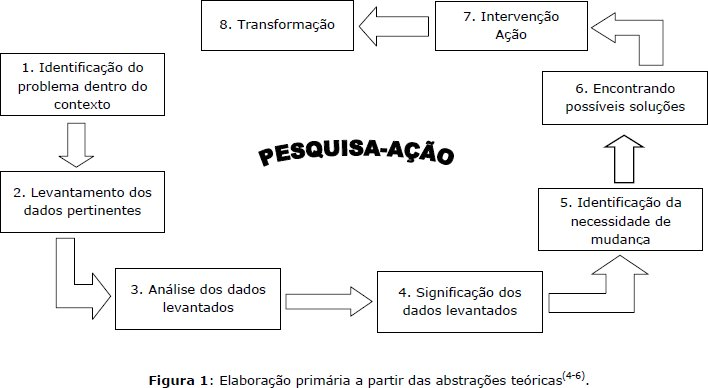
\includegraphics[width=\textwidth]{ProjetoII/pesquisa-acao}

  Fonte: Koerich {\em et al}, 2009.
\end{frame}

\section{Resultados}

\subsection{Resultados esperados}

\begin{frame}{Resultados esperados}
  \begin{itemize}
  \item Confirmação ou refutação das hipóteses descritas
  \item Inferência de causalidade entre variáveis
  \item Divulgação e publicação de relatório, artigo, congresso,
    dissertação, tese, etc.
  \item Obtenção de titulação {\em stricto sensu} ou {\em lato sensu}
  \end{itemize}
\end{frame}

\subsection{Resultados preliminares}

\begin{frame}{Resultados preliminares}
  Caso disponíveis, resultados preliminares devem ser descritos para:
  \begin{itemize}
  \item Validar a metodologia
  \item Indicar o rumo da pesquisa (qualidade)
  \item Testar (preliminarmente) a análise:
    \begin{itemize}
    \item dos dados
    \item das hipóteses
    \end{itemize}
  \item Transmitir confiança aos avaliadores (prazo)
  \end{itemize}
\end{frame}

\begin{frame}{Resultados preliminares}
  Podem ser descritos:
  \begin{itemize}
  \item Em uma coleta preliminar, em pequena escala (piloto)
  \item Em um estágio inicial da coleta
  \item Após a coleta completa, mas análise de um subconjunto dos dados
  \end{itemize}
\end{frame}

\section{Sumários}

\subsection{Sumário do Projeto}

\begin{frame}{Sumário do projeto}
  \begin{itemize}
  \item Utilizar as ferramentas automáticas do software escolhido
    (Word, LibreOffice, \LaTeX, etc.)
  \item Formatar seções selecionando os {\bf estilos de texto}
    (ex. Título 1, Título 2, \ldots)
  \item \alert{Nunca} formatar seções manualmente!
  \item Indicar seções primárias, secundárias e terciárias
  \item (ABNT) Primárias em caixa alta, secundárias (em diante)
    capitalizadas
  \end{itemize}
\end{frame}

\begin{frame}{Exemplo}
  \begin{center}
    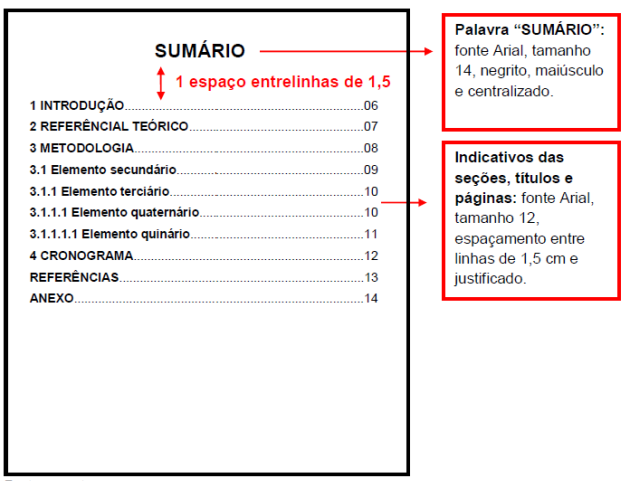
\includegraphics[height=0.8\textheight]{ProjetoII/sumario}
  \end{center}

  Fonte: \url{http://fio.edu.br/manualtcc/co/4_Sumario.html}
\end{frame}

\subsection{Lista de abreviaturas}

\begin{frame}{Lista de abreviaturas}
  \begin{itemize}
  \item Indicar \alert{todas} as abreviaturas utilizadas no texto
    (mesmo que uma única vez)
  \item Ordem alfabética das abreviaturas
  \item (ABNT) Sigla em caixa alta, significado capitalizado
  \end{itemize}
\end{frame}

\begin{frame}{Exemplo}
  \begin{center}
    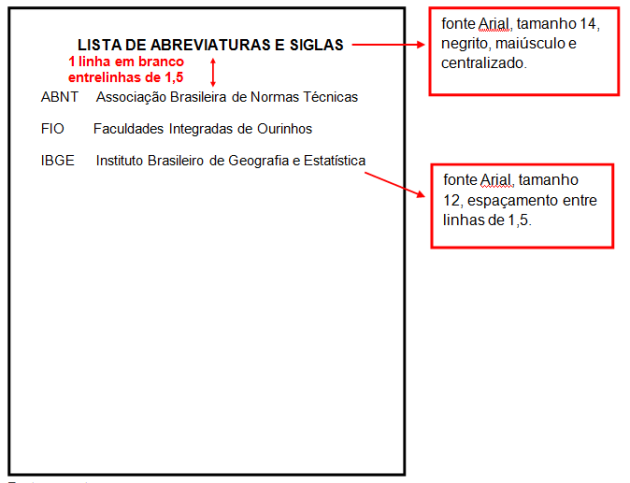
\includegraphics[height=0.8\textheight]{ProjetoII/lista_abreviaturas}
  \end{center}

  Fonte: \url{http://fio.edu.br/manualtcc/co/15_Lista_de_abreviaturas.html}
\end{frame}

\subsection{Listas de Figuras e Tabelas}

\begin{frame}{Listas de Figuras e de Tabelas}
  \begin{itemize}
  \item Legendas das figuras e tabelas, com o número de página em que
    aparecem
  \item Utilizar ferramentas automáticas (Inserir Figura/Tabela,
    Propriedades/Legenda).
  \item (opcional) versão resumida da legenda, caso muito longa
  \end{itemize}
\end{frame}

\begin{frame}{Exemplo}
  \begin{center}
    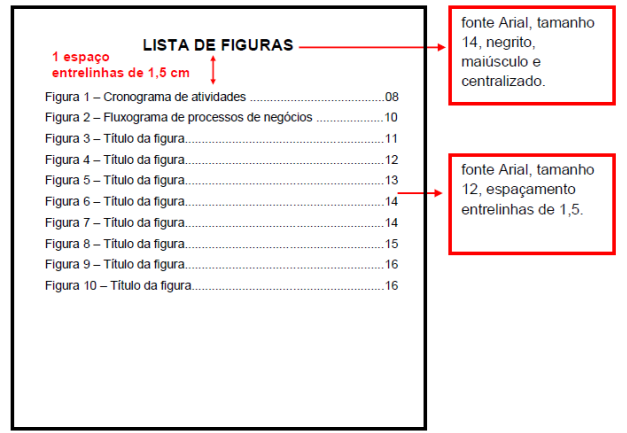
\includegraphics[height=0.8\textheight]{ProjetoII/lista_figuras}
  \end{center}

  Fonte: \url{http://fio.edu.br/manualtcc/co/13_Lista_de_ilustracoes.html}
\end{frame}

\section{Referências}

\begin{frame}{Referências}
  \begin{itemize}
  \item<1-> VEduca:
    \url{http://www.veduca.com.br/assistir/metodologia-cientifica}
  \item<1-> Koerich {\em et al} (2009): Pesquisa-ação: ferramenta
    metodológica para a pesquisa qualitativa (Rev. Eletr. Enf.)
    \url{https://www.fen.ufg.br/fen_revista/v11/n3/v11n3a33.htm}
  \item<1-> Prodanov (2013): cap 4.
  \item<1-> Lakatos (2003): cap 10.
  \end{itemize}
\end{frame}

\end{document}
